\documentclass[1p]{elsarticle_modified}
%\bibliographystyle{elsarticle-num}

%\usepackage[colorlinks]{hyperref}
%\usepackage{abbrmath_seonhwa} %\Abb, \Ascr, \Acal ,\Abf, \Afrak
\usepackage{amsfonts}
\usepackage{amssymb}
\usepackage{amsmath}
\usepackage{amsthm}
\usepackage{scalefnt}
\usepackage{amsbsy}
\usepackage{kotex}
\usepackage{caption}
\usepackage{subfig}
\usepackage{color}
\usepackage{graphicx}
\usepackage{xcolor} %% white, black, red, green, blue, cyan, magenta, yellow
\usepackage{float}
\usepackage{setspace}
\usepackage{hyperref}

\usepackage{tikz}
\usetikzlibrary{arrows}

\usepackage{multirow}
\usepackage{array} % fixed length table
\usepackage{hhline}

%%%%%%%%%%%%%%%%%%%%%
\makeatletter
\renewcommand*\env@matrix[1][\arraystretch]{%
	\edef\arraystretch{#1}%
	\hskip -\arraycolsep
	\let\@ifnextchar\new@ifnextchar
	\array{*\c@MaxMatrixCols c}}
\makeatother %https://tex.stackexchange.com/questions/14071/how-can-i-increase-the-line-spacing-in-a-matrix
%%%%%%%%%%%%%%%

\usepackage[normalem]{ulem}

\newcommand{\msout}[1]{\ifmmode\text{\sout{\ensuremath{#1}}}\else\sout{#1}\fi}
%SOURCE: \msout is \stkout macro in https://tex.stackexchange.com/questions/20609/strikeout-in-math-mode

\newcommand{\cancel}[1]{
	\ifmmode
	{\color{red}\msout{#1}}
	\else
	{\color{red}\sout{#1}}
	\fi
}

\newcommand{\add}[1]{
	{\color{blue}\uwave{#1}}
}

\newcommand{\replace}[2]{
	\ifmmode
	{\color{red}\msout{#1}}{\color{blue}\uwave{#2}}
	\else
	{\color{red}\sout{#1}}{\color{blue}\uwave{#2}}
	\fi
}

\newcommand{\Sol}{\mathcal{S}} %segment
\newcommand{\D}{D} %diagram
\newcommand{\A}{\mathcal{A}} %arc


%%%%%%%%%%%%%%%%%%%%%%%%%%%%%5 test

\def\sl{\operatorname{\textup{SL}}(2,\Cbb)}
\def\psl{\operatorname{\textup{PSL}}(2,\Cbb)}
\def\quan{\mkern 1mu \triangleright \mkern 1mu}

\theoremstyle{definition}
\newtheorem{thm}{Theorem}[section]
\newtheorem{prop}[thm]{Proposition}
\newtheorem{lem}[thm]{Lemma}
\newtheorem{ques}[thm]{Question}
\newtheorem{cor}[thm]{Corollary}
\newtheorem{defn}[thm]{Definition}
\newtheorem{exam}[thm]{Example}
\newtheorem{rmk}[thm]{Remark}
\newtheorem{alg}[thm]{Algorithm}

\newcommand{\I}{\sqrt{-1}}
\begin{document}

%\begin{frontmatter}
%
%\title{Boundary parabolic representations of knots up to 8 crossings}
%
%%% Group authors per affiliation:
%\author{Yunhi Cho} 
%\address{Department of Mathematics, University of Seoul, Seoul, Korea}
%\ead{yhcho@uos.ac.kr}
%
%
%\author{Seonhwa Kim} %\fnref{s_kim}}
%\address{Center for Geometry and Physics, Institute for Basic Science, Pohang, 37673, Korea}
%\ead{ryeona17@ibs.re.kr}
%
%\author{Hyuk Kim}
%\address{Department of Mathematical Sciences, Seoul National University, Seoul 08826, Korea}
%\ead{hyukkim@snu.ac.kr}
%
%\author{Seokbeom Yoon}
%\address{Department of Mathematical Sciences, Seoul National University, Seoul, 08826,  Korea}
%\ead{sbyoon15@snu.ac.kr}
%
%\begin{abstract}
%We find all boundary parabolic representation of knots up to 8 crossings.
%
%\end{abstract}
%\begin{keyword}
%    \MSC[2010] 57M25 
%\end{keyword}
%
%\end{frontmatter}

%\linenumbers
%\tableofcontents
%
\newcommand\colored[1]{\textcolor{white}{\rule[-0.35ex]{0.8em}{1.4ex}}\kern-0.8em\color{red} #1}%
%\newcommand\colored[1]{\textcolor{white}{ #1}\kern-2.17ex	\textcolor{white}{ #1}\kern-1.81ex	\textcolor{white}{ #1}\kern-2.15ex\color{red}#1	}

{\Large $\underline{12n_{0040}~(K12n_{0040})}$}

\setlength{\tabcolsep}{10pt}
\renewcommand{\arraystretch}{1.6}
\vspace{1cm}\begin{tabular}{m{100pt}>{\centering\arraybackslash}m{274pt}}
\multirow{5}{120pt}{
	\centering
	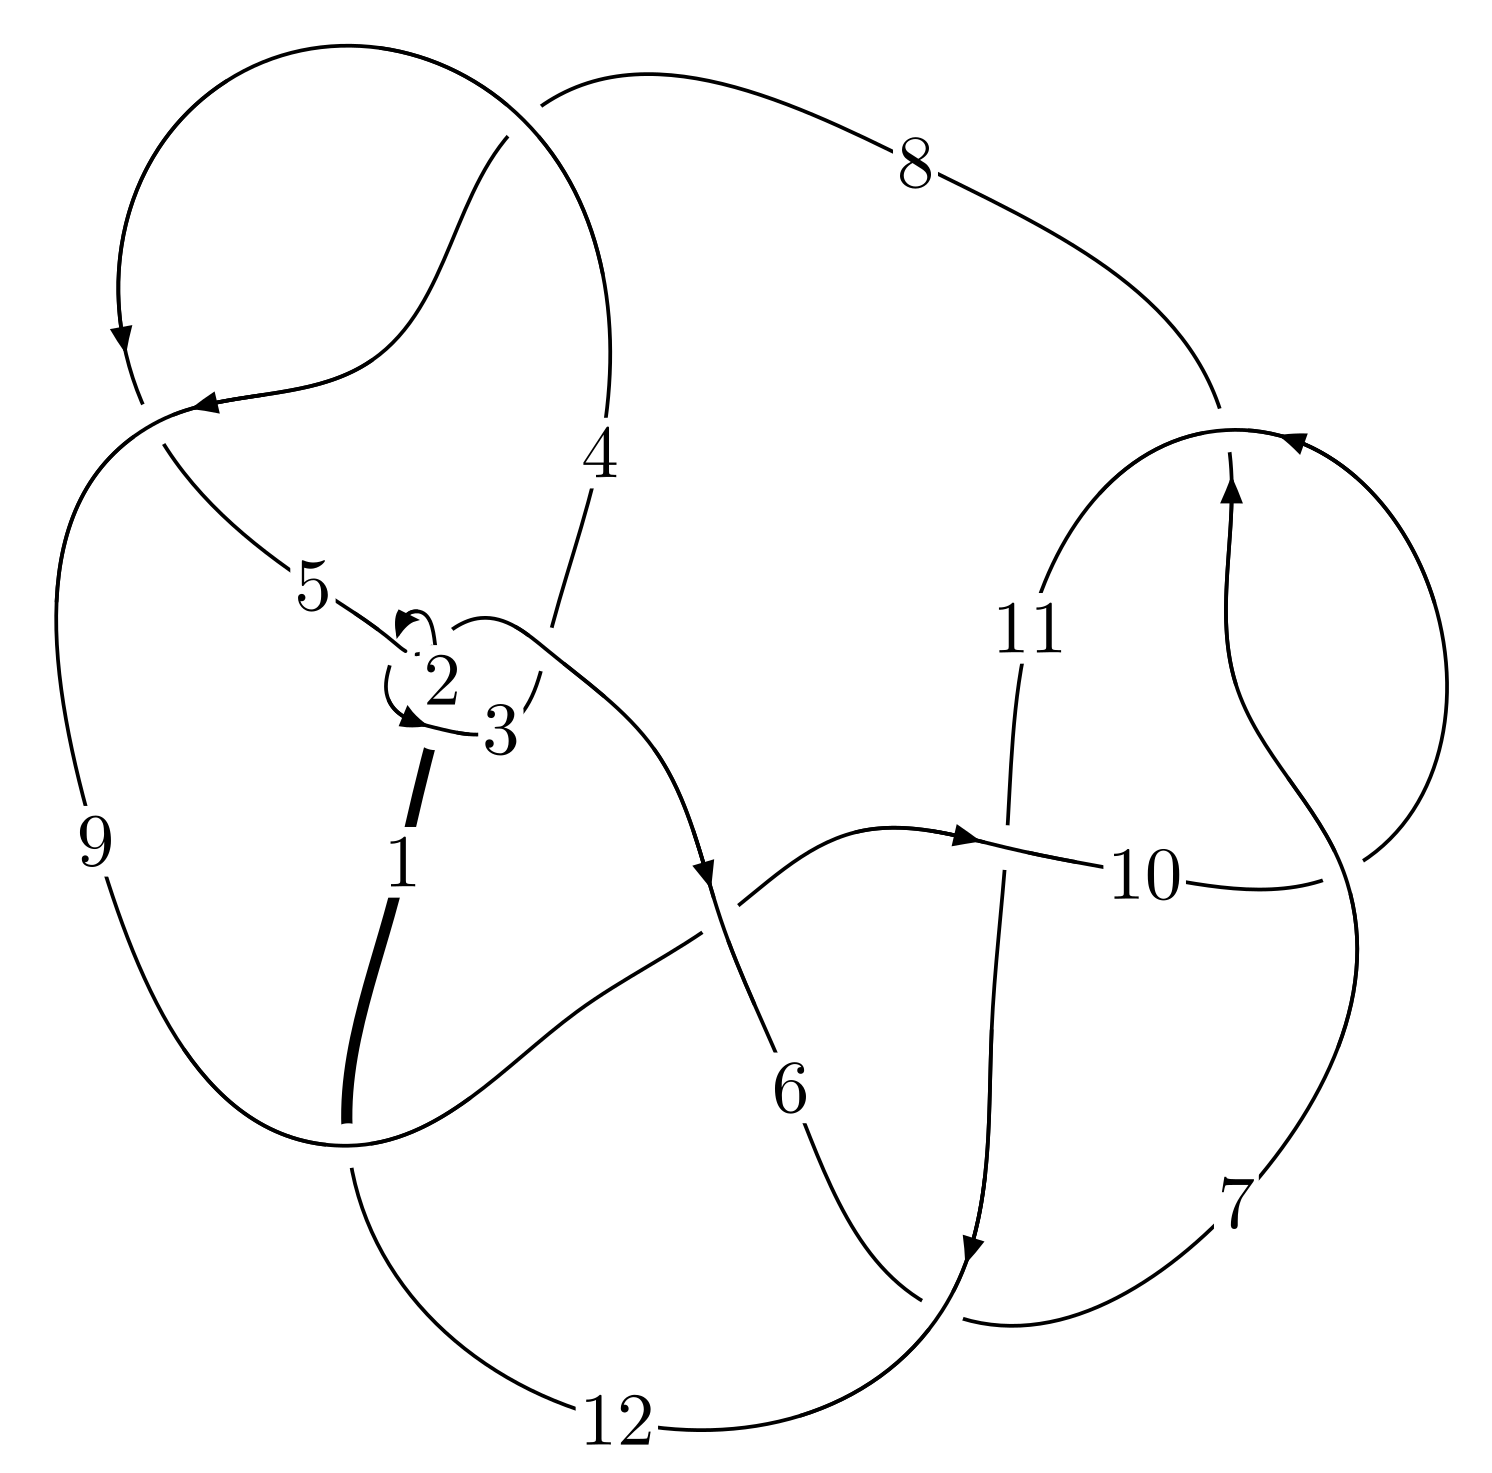
\includegraphics[width=112pt]{../../../GIT/diagram.site/Diagrams/png/2129_12n_0040.png}\\
\ \ \ A knot diagram\footnotemark}&
\allowdisplaybreaks
\textbf{Linearized knot diagam} \\
\cline{2-2}
 &
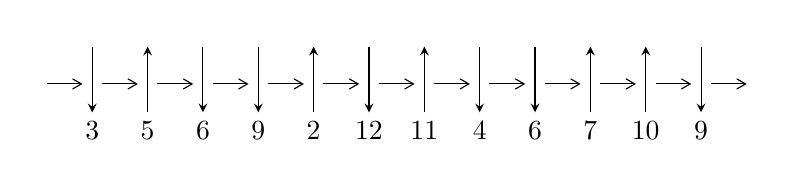
\begin{tikzpicture}[x=20pt, y=17pt]
	% nodes
	\node (C0) at (0, 0) {};
	\node (C1) at (1, 0) {};
	\node (C1U) at (1, +1) {};
	\node (C1D) at (1, -1) {3};

	\node (C2) at (2, 0) {};
	\node (C2U) at (2, +1) {};
	\node (C2D) at (2, -1) {5};

	\node (C3) at (3, 0) {};
	\node (C3U) at (3, +1) {};
	\node (C3D) at (3, -1) {6};

	\node (C4) at (4, 0) {};
	\node (C4U) at (4, +1) {};
	\node (C4D) at (4, -1) {9};

	\node (C5) at (5, 0) {};
	\node (C5U) at (5, +1) {};
	\node (C5D) at (5, -1) {2};

	\node (C6) at (6, 0) {};
	\node (C6U) at (6, +1) {};
	\node (C6D) at (6, -1) {12};

	\node (C7) at (7, 0) {};
	\node (C7U) at (7, +1) {};
	\node (C7D) at (7, -1) {11};

	\node (C8) at (8, 0) {};
	\node (C8U) at (8, +1) {};
	\node (C8D) at (8, -1) {4};

	\node (C9) at (9, 0) {};
	\node (C9U) at (9, +1) {};
	\node (C9D) at (9, -1) {6};

	\node (C10) at (10, 0) {};
	\node (C10U) at (10, +1) {};
	\node (C10D) at (10, -1) {7};

	\node (C11) at (11, 0) {};
	\node (C11U) at (11, +1) {};
	\node (C11D) at (11, -1) {10};

	\node (C12) at (12, 0) {};
	\node (C12U) at (12, +1) {};
	\node (C12D) at (12, -1) {9};
	\node (C13) at (13, 0) {};

	% arrows
	\draw[->,>={angle 60}]
	(C0) edge (C1) (C1) edge (C2) (C2) edge (C3) (C3) edge (C4) (C4) edge (C5) (C5) edge (C6) (C6) edge (C7) (C7) edge (C8) (C8) edge (C9) (C9) edge (C10) (C10) edge (C11) (C11) edge (C12) (C12) edge (C13) ;	\draw[->,>=stealth]
	(C1U) edge (C1D) (C2D) edge (C2U) (C3U) edge (C3D) (C4U) edge (C4D) (C5D) edge (C5U) (C6U) edge (C6D) (C7D) edge (C7U) (C8U) edge (C8D) (C9U) edge (C9D) (C10D) edge (C10U) (C11D) edge (C11U) (C12U) edge (C12D) ;
	\end{tikzpicture} \\
\hhline{~~} \\& 
\textbf{Solving Sequence} \\ \cline{2-2} 
 &
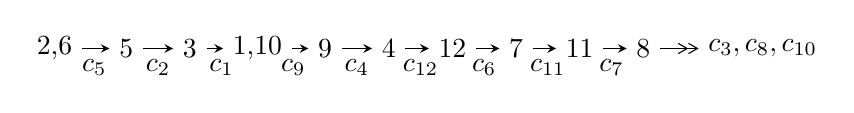
\begin{tikzpicture}[x=23pt, y=7pt]
	% node
	\node (A0) at (-1/8, 0) {2,6};
	\node (A1) at (1, 0) {5};
	\node (A2) at (2, 0) {3};
	\node (A3) at (49/16, 0) {1,10};
	\node (A4) at (33/8, 0) {9};
	\node (A5) at (41/8, 0) {4};
	\node (A6) at (49/8, 0) {12};
	\node (A7) at (57/8, 0) {7};
	\node (A8) at (65/8, 0) {11};
	\node (A9) at (73/8, 0) {8};
	\node (C1) at (1/2, -1) {$c_{5}$};
	\node (C2) at (3/2, -1) {$c_{2}$};
	\node (C3) at (5/2, -1) {$c_{1}$};
	\node (C4) at (29/8, -1) {$c_{9}$};
	\node (C5) at (37/8, -1) {$c_{4}$};
	\node (C6) at (45/8, -1) {$c_{12}$};
	\node (C7) at (53/8, -1) {$c_{6}$};
	\node (C8) at (61/8, -1) {$c_{11}$};
	\node (C9) at (69/8, -1) {$c_{7}$};
	\node (A10) at (11, 0) {$c_{3},c_{8},c_{10}$};

	% edge
	\draw[->,>=stealth]	
	(A0) edge (A1) (A1) edge (A2) (A2) edge (A3) (A3) edge (A4) (A4) edge (A5) (A5) edge (A6) (A6) edge (A7) (A7) edge (A8) (A8) edge (A9) ;
	\draw[->>,>={angle 60}]	
	(A9) edge (A10);
\end{tikzpicture} \\ 

\end{tabular} \\

\footnotetext{
The image of knot diagram is generated by the software ``\textbf{Draw programme}" developed by Andrew Bartholomew(\url{http://www.layer8.co.uk/maths/draw/index.htm\#Running-draw}), where we modified some parts for our purpose(\url{https://github.com/CATsTAILs/LinksPainter}).
}\phantom \\ \newline 
\centering \textbf{Ideals for irreducible components\footnotemark of $X_{\text{par}}$} 
 
\begin{align*}
I^u_{1}&=\langle 
34 u^{42}+241 u^{41}+\cdots+32 b+95,\;27 u^{42}+149 u^{41}+\cdots+32 a+121,\;u^{43}+7 u^{42}+\cdots+8 u+1\rangle \\
I^u_{2}&=\langle 
- a u+3 b+2 a,\;a^6- a^5 u- a^5-3 a^4 u+12 a^3 u-6 a^3-9 a u+18 a-27,\;u^2- u+1\rangle \\
\\
\end{align*}
\raggedright * 2 irreducible components of $\dim_{\mathbb{C}}=0$, with total 55 representations.\\
\footnotetext{All coefficients of polynomials are rational numbers. But the coefficients are sometimes approximated in decimal forms when there is not enough margin.}
\newpage
\renewcommand{\arraystretch}{1}
\centering \section*{I. $I^u_{1}= \langle 34 u^{42}+241 u^{41}+\cdots+32 b+95,\;27 u^{42}+149 u^{41}+\cdots+32 a+121,\;u^{43}+7 u^{42}+\cdots+8 u+1 \rangle$}
\flushleft \textbf{(i) Arc colorings}\\
\begin{tabular}{m{7pt} m{180pt} m{7pt} m{180pt} }
\flushright $a_{2}=$&$\begin{pmatrix}0\\u\end{pmatrix}$ \\
\flushright $a_{6}=$&$\begin{pmatrix}1\\0\end{pmatrix}$ \\
\flushright $a_{5}=$&$\begin{pmatrix}1\\u^2\end{pmatrix}$ \\
\flushright $a_{3}=$&$\begin{pmatrix}u\\u^3+u\end{pmatrix}$ \\
\flushright $a_{1}=$&$\begin{pmatrix}u^3\\u^5+u^3+u\end{pmatrix}$ \\
\flushright $a_{10}=$&$\begin{pmatrix}-0.843750 u^{42}-4.65625 u^{41}+\cdots-25.8125 u-3.78125\\-1.06250 u^{42}-7.53125 u^{41}+\cdots-14.0313 u-2.96875\end{pmatrix}$ \\
\flushright $a_{9}=$&$\begin{pmatrix}-1.90625 u^{42}-12.1875 u^{41}+\cdots-39.8438 u-6.75000\\-1.06250 u^{42}-7.53125 u^{41}+\cdots-14.0313 u-2.96875\end{pmatrix}$ \\
\flushright $a_{4}=$&$\begin{pmatrix}- u^3\\u^3+u\end{pmatrix}$ \\
\flushright $a_{12}=$&$\begin{pmatrix}0.0312500 u^{41}+0.187500 u^{40}+\cdots+0.218750 u-0.968750\\-\frac{1}{32} u^{42}-\frac{7}{32} u^{41}+\cdots+\frac{7}{4} u-\frac{1}{32}\end{pmatrix}$ \\
\flushright $a_{7}=$&$\begin{pmatrix}-0.156250 u^{42}-0.687500 u^{41}+\cdots+0.0312500 u+1.31250\\-0.281250 u^{42}-2.09375 u^{41}+\cdots-3.18750 u-0.406250\end{pmatrix}$ \\
\flushright $a_{11}=$&$\begin{pmatrix}-0.125000 u^{42}-1.53125 u^{41}+\cdots-3.09375 u-0.843750\\0.281250 u^{42}+2.15625 u^{41}+\cdots+4.62500 u+0.468750\end{pmatrix}$ \\
\flushright $a_{8}=$&$\begin{pmatrix}1.28125 u^{42}+9.50000 u^{41}+\cdots+47.5313 u+7.81250\\0.875000 u^{42}+5.59375 u^{41}+\cdots+9.15625 u+2.03125\end{pmatrix}$\\&\end{tabular}
\flushleft \textbf{(ii) Obstruction class $= -1$}\\~\\
\flushleft \textbf{(iii) Cusp Shapes $= -\frac{21}{4} u^{42}-\frac{619}{16} u^{41}+\cdots-\frac{887}{8} u-\frac{183}{8}$}\\~\\
\newpage\renewcommand{\arraystretch}{1}
\flushleft \textbf{(iv) u-Polynomials at the component}\newline \\
\begin{tabular}{m{50pt}|m{274pt}}
Crossings & \hspace{64pt}u-Polynomials at each crossing \\
\hline $$\begin{aligned}c_{1}\end{aligned}$$&$\begin{aligned}
&u^{43}+29 u^{42}+\cdots-6 u-1
\end{aligned}$\\
\hline $$\begin{aligned}c_{2},c_{5}\end{aligned}$$&$\begin{aligned}
&u^{43}+7 u^{42}+\cdots+8 u+1
\end{aligned}$\\
\hline $$\begin{aligned}c_{3}\end{aligned}$$&$\begin{aligned}
&u^{43}-7 u^{42}+\cdots-15 u+2
\end{aligned}$\\
\hline $$\begin{aligned}c_{4},c_{8}\end{aligned}$$&$\begin{aligned}
&u^{43}- u^{42}+\cdots+4096 u+4096
\end{aligned}$\\
\hline $$\begin{aligned}c_{6}\end{aligned}$$&$\begin{aligned}
&u^{43}-9 u^{42}+\cdots+301 u-32
\end{aligned}$\\
\hline $$\begin{aligned}c_{7},c_{10}\end{aligned}$$&$\begin{aligned}
&u^{43}-3 u^{42}+\cdots-4 u+1
\end{aligned}$\\
\hline $$\begin{aligned}c_{9}\end{aligned}$$&$\begin{aligned}
&u^{43}+3 u^{42}+\cdots+u^2+1
\end{aligned}$\\
\hline $$\begin{aligned}c_{11}\end{aligned}$$&$\begin{aligned}
&u^{43}-19 u^{42}+\cdots-2 u-1
\end{aligned}$\\
\hline $$\begin{aligned}c_{12}\end{aligned}$$&$\begin{aligned}
&u^{43}-13 u^{42}+\cdots-396502 u-27289
\end{aligned}$\\
\hline
\end{tabular}\\~\\
\newpage\renewcommand{\arraystretch}{1}
\flushleft \textbf{(v) Riley Polynomials at the component}\newline \\
\begin{tabular}{m{50pt}|m{274pt}}
Crossings & \hspace{64pt}Riley Polynomials at each crossing \\
\hline $$\begin{aligned}c_{1}\end{aligned}$$&$\begin{aligned}
&y^{43}-23 y^{42}+\cdots-70 y-1
\end{aligned}$\\
\hline $$\begin{aligned}c_{2},c_{5}\end{aligned}$$&$\begin{aligned}
&y^{43}+29 y^{42}+\cdots-6 y-1
\end{aligned}$\\
\hline $$\begin{aligned}c_{3}\end{aligned}$$&$\begin{aligned}
&y^{43}-75 y^{42}+\cdots+109 y-4
\end{aligned}$\\
\hline $$\begin{aligned}c_{4},c_{8}\end{aligned}$$&$\begin{aligned}
&y^{43}-65 y^{42}+\cdots+150994944 y-16777216
\end{aligned}$\\
\hline $$\begin{aligned}c_{6}\end{aligned}$$&$\begin{aligned}
&y^{43}-7 y^{42}+\cdots+2985 y-1024
\end{aligned}$\\
\hline $$\begin{aligned}c_{7},c_{10}\end{aligned}$$&$\begin{aligned}
&y^{43}-19 y^{42}+\cdots-2 y-1
\end{aligned}$\\
\hline $$\begin{aligned}c_{9}\end{aligned}$$&$\begin{aligned}
&y^{43}-59 y^{42}+\cdots-2 y-1
\end{aligned}$\\
\hline $$\begin{aligned}c_{11}\end{aligned}$$&$\begin{aligned}
&y^{43}+13 y^{42}+\cdots-54 y-1
\end{aligned}$\\
\hline $$\begin{aligned}c_{12}\end{aligned}$$&$\begin{aligned}
&y^{43}-119 y^{42}+\cdots-1101094234046 y-744689521
\end{aligned}$\\
\hline
\end{tabular}\\~\\
\newpage\flushleft \textbf{(vi) Complex Volumes and Cusp Shapes}
$$\begin{array}{c|c|c}  
\text{Solutions to }I^u_{1}& \I (\text{vol} + \sqrt{-1}CS) & \text{Cusp shape}\\
 \hline 
\begin{aligned}
u &= -0.108850 + 1.019930 I \\
a &= -2.54446 - 0.82403 I \\
b &= \phantom{-}0.887627 + 0.888202 I\end{aligned}
 & \phantom{-}0.432070 - 0.070776 I & -2.00000 + 0. I\phantom{ +0.000000I} \\ \hline\begin{aligned}
u &= -0.108850 - 1.019930 I \\
a &= -2.54446 + 0.82403 I \\
b &= \phantom{-}0.887627 - 0.888202 I\end{aligned}
 & \phantom{-}0.432070 + 0.070776 I & -2.00000 + 0. I\phantom{ +0.000000I} \\ \hline\begin{aligned}
u &= -1.03310\phantom{ +0.000000I} \\
a &= \phantom{-}1.81625\phantom{ +0.000000I} \\
b &= -1.75986\phantom{ +0.000000I}\end{aligned}
 & -5.16147\phantom{ +0.000000I} & \phantom{-}0.303180\phantom{ +0.000000I} \\ \hline\begin{aligned}
u &= \phantom{-}0.631242 + 0.697176 I \\
a &= -0.026925 + 1.068100 I \\
b &= \phantom{-}0.114579 - 0.360320 I\end{aligned}
 & \phantom{-}1.44756 + 4.15054 I & -1.66670 - 7.98021 I \\ \hline\begin{aligned}
u &= \phantom{-}0.631242 - 0.697176 I \\
a &= -0.026925 - 1.068100 I \\
b &= \phantom{-}0.114579 + 0.360320 I\end{aligned}
 & \phantom{-}1.44756 - 4.15054 I & -1.66670 + 7.98021 I \\ \hline\begin{aligned}
u &= \phantom{-}0.630221 + 0.873340 I \\
a &= \phantom{-}0.381127 - 0.768103 I \\
b &= -0.219981 + 0.236881 I\end{aligned}
 & \phantom{-}0.968100 + 0.793721 I & \phantom{-0.000000 } 0 \\ \hline\begin{aligned}
u &= \phantom{-}0.630221 - 0.873340 I \\
a &= \phantom{-}0.381127 + 0.768103 I \\
b &= -0.219981 - 0.236881 I\end{aligned}
 & \phantom{-}0.968100 - 0.793721 I & \phantom{-0.000000 } 0 \\ \hline\begin{aligned}
u &= -1.093460 + 0.077172 I \\
a &= \phantom{-}1.96976 - 0.17734 I \\
b &= -1.81042 + 0.05602 I\end{aligned}
 & -9.35130 + 7.40339 I & \phantom{-0.000000 } 0. - 4.50100 I \\ \hline\begin{aligned}
u &= -1.093460 - 0.077172 I \\
a &= \phantom{-}1.96976 + 0.17734 I \\
b &= -1.81042 - 0.05602 I\end{aligned}
 & -9.35130 - 7.40339 I & \phantom{-0.000000 -}0. + 4.50100 I \\ \hline\begin{aligned}
u &= \phantom{-}0.356528 + 0.829227 I \\
a &= -0.809224 - 0.565549 I \\
b &= \phantom{-}0.200199 + 0.315601 I\end{aligned}
 & -0.32126 + 1.54787 I & -2.12659 - 4.62507 I\\
 \hline 
 \end{array}$$\newpage$$\begin{array}{c|c|c}  
\text{Solutions to }I^u_{1}& \I (\text{vol} + \sqrt{-1}CS) & \text{Cusp shape}\\
 \hline 
\begin{aligned}
u &= \phantom{-}0.356528 - 0.829227 I \\
a &= -0.809224 + 0.565549 I \\
b &= \phantom{-}0.200199 - 0.315601 I\end{aligned}
 & -0.32126 - 1.54787 I & -2.12659 + 4.62507 I \\ \hline\begin{aligned}
u &= -1.097840 + 0.043281 I \\
a &= -1.97365 + 0.09899 I \\
b &= \phantom{-}1.81083 - 0.03124 I\end{aligned}
 & -11.14880 + 1.85775 I & \phantom{-0.000000 } 0 \\ \hline\begin{aligned}
u &= -1.097840 - 0.043281 I \\
a &= -1.97365 - 0.09899 I \\
b &= \phantom{-}1.81083 + 0.03124 I\end{aligned}
 & -11.14880 - 1.85775 I & \phantom{-0.000000 } 0 \\ \hline\begin{aligned}
u &= -0.231681 + 1.107840 I \\
a &= -3.17472 - 0.52343 I \\
b &= \phantom{-}1.31188 + 0.91141 I\end{aligned}
 & -1.74448 - 7.62411 I & \phantom{-0.000000 } 0 \\ \hline\begin{aligned}
u &= -0.231681 - 1.107840 I \\
a &= -3.17472 + 0.52343 I \\
b &= \phantom{-}1.31188 - 0.91141 I\end{aligned}
 & -1.74448 + 7.62411 I & \phantom{-0.000000 } 0 \\ \hline\begin{aligned}
u &= \phantom{-}0.441020 + 1.047300 I \\
a &= -1.087770 + 0.250841 I \\
b &= \phantom{-}0.447924 + 0.048017 I\end{aligned}
 & -1.10611 + 1.42382 I & \phantom{-0.000000 } 0 \\ \hline\begin{aligned}
u &= \phantom{-}0.441020 - 1.047300 I \\
a &= -1.087770 - 0.250841 I \\
b &= \phantom{-}0.447924 - 0.048017 I\end{aligned}
 & -1.10611 - 1.42382 I & \phantom{-0.000000 } 0 \\ \hline\begin{aligned}
u &= -0.173823 + 1.139560 I \\
a &= \phantom{-}2.91930 + 0.38726 I \\
b &= -1.21169 - 0.76310 I\end{aligned}
 & -4.07750 - 2.66673 I & \phantom{-0.000000 } 0 \\ \hline\begin{aligned}
u &= -0.173823 - 1.139560 I \\
a &= \phantom{-}2.91930 - 0.38726 I \\
b &= -1.21169 + 0.76310 I\end{aligned}
 & -4.07750 + 2.66673 I & \phantom{-0.000000 } 0 \\ \hline\begin{aligned}
u &= \phantom{-}0.555429 + 1.053250 I \\
a &= \phantom{-}0.937490 - 0.560097 I \\
b &= -0.423819 + 0.102545 I\end{aligned}
 & -0.20886 + 5.67924 I & \phantom{-0.000000 } 0\\
 \hline 
 \end{array}$$\newpage$$\begin{array}{c|c|c}  
\text{Solutions to }I^u_{1}& \I (\text{vol} + \sqrt{-1}CS) & \text{Cusp shape}\\
 \hline 
\begin{aligned}
u &= \phantom{-}0.555429 - 1.053250 I \\
a &= \phantom{-}0.937490 + 0.560097 I \\
b &= -0.423819 - 0.102545 I\end{aligned}
 & -0.20886 - 5.67924 I & \phantom{-0.000000 } 0 \\ \hline\begin{aligned}
u &= -0.013036 + 1.234440 I \\
a &= \phantom{-}2.43278 + 0.00691 I \\
b &= -1.046990 - 0.429320 I\end{aligned}
 & -5.51855 - 0.23082 I & \phantom{-0.000000 } 0 \\ \hline\begin{aligned}
u &= -0.013036 - 1.234440 I \\
a &= \phantom{-}2.43278 - 0.00691 I \\
b &= -1.046990 + 0.429320 I\end{aligned}
 & -5.51855 + 0.23082 I & \phantom{-0.000000 } 0 \\ \hline\begin{aligned}
u &= \phantom{-}0.067968 + 1.257240 I \\
a &= -2.24159 + 0.11300 I \\
b &= \phantom{-}0.972223 + 0.322115 I\end{aligned}
 & -4.39423 + 4.95924 I & \phantom{-0.000000 } 0 \\ \hline\begin{aligned}
u &= \phantom{-}0.067968 - 1.257240 I \\
a &= -2.24159 - 0.11300 I \\
b &= \phantom{-}0.972223 - 0.322115 I\end{aligned}
 & -4.39423 - 4.95924 I & \phantom{-0.000000 } 0 \\ \hline\begin{aligned}
u &= -0.51561 + 1.34254 I \\
a &= \phantom{-}3.53483 - 0.69986 I \\
b &= -1.90537 - 0.30670 I\end{aligned}
 & -9.34262 - 5.50773 I & \phantom{-0.000000 } 0 \\ \hline\begin{aligned}
u &= -0.51561 - 1.34254 I \\
a &= \phantom{-}3.53483 + 0.69986 I \\
b &= -1.90537 + 0.30670 I\end{aligned}
 & -9.34262 + 5.50773 I & \phantom{-0.000000 } 0 \\ \hline\begin{aligned}
u &= -0.57404 + 1.34689 I \\
a &= \phantom{-}3.56336 - 0.81250 I \\
b &= -1.96829 - 0.24490 I\end{aligned}
 & -13.3037 - 13.3388 I & \phantom{-0.000000 } 0 \\ \hline\begin{aligned}
u &= -0.57404 - 1.34689 I \\
a &= \phantom{-}3.56336 + 0.81250 I \\
b &= -1.96829 + 0.24490 I\end{aligned}
 & -13.3037 + 13.3388 I & \phantom{-0.000000 } 0 \\ \hline\begin{aligned}
u &= -0.029590 + 0.530131 I \\
a &= \phantom{-}1.15627 + 1.68061 I \\
b &= \phantom{-}0.135978 - 0.751914 I\end{aligned}
 & \phantom{-}1.74801 - 1.44634 I & \phantom{-}0.320350 + 0.404730 I\\
 \hline 
 \end{array}$$\newpage$$\begin{array}{c|c|c}  
\text{Solutions to }I^u_{1}& \I (\text{vol} + \sqrt{-1}CS) & \text{Cusp shape}\\
 \hline 
\begin{aligned}
u &= -0.029590 - 0.530131 I \\
a &= \phantom{-}1.15627 - 1.68061 I \\
b &= \phantom{-}0.135978 + 0.751914 I\end{aligned}
 & \phantom{-}1.74801 + 1.44634 I & \phantom{-}0.320350 - 0.404730 I \\ \hline\begin{aligned}
u &= -0.55869 + 1.36236 I \\
a &= -3.52852 + 0.79270 I \\
b &= \phantom{-}1.93730 + 0.24369 I\end{aligned}
 & -15.2690 - 7.7521 I & \phantom{-0.000000 } 0 \\ \hline\begin{aligned}
u &= -0.55869 - 1.36236 I \\
a &= -3.52852 - 0.79270 I \\
b &= \phantom{-}1.93730 - 0.24369 I\end{aligned}
 & -15.2690 + 7.7521 I & \phantom{-0.000000 } 0 \\ \hline\begin{aligned}
u &= -0.50713 + 1.39889 I \\
a &= -3.43056 + 0.73543 I \\
b &= \phantom{-}1.84983 + 0.24468 I\end{aligned}
 & -15.7130 - 3.8589 I & \phantom{-0.000000 } 0 \\ \hline\begin{aligned}
u &= -0.50713 - 1.39889 I \\
a &= -3.43056 - 0.73543 I \\
b &= \phantom{-}1.84983 - 0.24468 I\end{aligned}
 & -15.7130 + 3.8589 I & \phantom{-0.000000 } 0 \\ \hline\begin{aligned}
u &= -0.48108 + 1.40912 I \\
a &= \phantom{-}3.38956 - 0.70682 I \\
b &= -1.81208 - 0.24952 I\end{aligned}
 & -14.0896 + 1.7953 I & \phantom{-0.000000 } 0 \\ \hline\begin{aligned}
u &= -0.48108 - 1.40912 I \\
a &= \phantom{-}3.38956 + 0.70682 I \\
b &= -1.81208 + 0.24952 I\end{aligned}
 & -14.0896 - 1.7953 I & \phantom{-0.000000 } 0 \\ \hline\begin{aligned}
u &= \phantom{-}0.395813 + 0.305739 I \\
a &= \phantom{-}0.39533 + 1.71062 I \\
b &= \phantom{-}0.047086 - 0.461449 I\end{aligned}
 & \phantom{-}1.64146 - 1.44258 I & \phantom{-}1.62393 + 1.37217 I \\ \hline\begin{aligned}
u &= \phantom{-}0.395813 - 0.305739 I \\
a &= \phantom{-}0.39533 - 1.71062 I \\
b &= \phantom{-}0.047086 + 0.461449 I\end{aligned}
 & \phantom{-}1.64146 + 1.44258 I & \phantom{-}1.62393 - 1.37217 I \\ \hline\begin{aligned}
u &= -0.355224 + 0.327355 I \\
a &= \phantom{-}0.46521 + 1.45996 I \\
b &= \phantom{-}0.831377 - 0.614700 I\end{aligned}
 & \phantom{-}0.49380 + 5.07125 I & -1.64078 - 7.14289 I\\
 \hline 
 \end{array}$$\newpage$$\begin{array}{c|c|c}  
\text{Solutions to }I^u_{1}& \I (\text{vol} + \sqrt{-1}CS) & \text{Cusp shape}\\
 \hline 
\begin{aligned}
u &= -0.355224 - 0.327355 I \\
a &= \phantom{-}0.46521 - 1.45996 I \\
b &= \phantom{-}0.831377 + 0.614700 I\end{aligned}
 & \phantom{-}0.49380 - 5.07125 I & -1.64078 + 7.14289 I \\ \hline\begin{aligned}
u &= -0.321614 + 0.162353 I \\
a &= -0.735715 - 0.820169 I \\
b &= -0.768263 + 0.294664 I\end{aligned}
 & -1.36971 + 0.61078 I & -6.09478 - 1.69888 I \\ \hline\begin{aligned}
u &= -0.321614 - 0.162353 I \\
a &= -0.735715 + 0.820169 I \\
b &= -0.768263 - 0.294664 I\end{aligned}
 & -1.36971 - 0.61078 I & -6.09478 + 1.69888 I\\
 \hline 
 \end{array}$$\newpage\newpage\renewcommand{\arraystretch}{1}
\centering \section*{II. $I^u_{2}= \langle - a u+3 b+2 a,\;- a^5 u-3 a^4 u+\cdots+18 a-27,\;u^2- u+1 \rangle$}
\flushleft \textbf{(i) Arc colorings}\\
\begin{tabular}{m{7pt} m{180pt} m{7pt} m{180pt} }
\flushright $a_{2}=$&$\begin{pmatrix}0\\u\end{pmatrix}$ \\
\flushright $a_{6}=$&$\begin{pmatrix}1\\0\end{pmatrix}$ \\
\flushright $a_{5}=$&$\begin{pmatrix}1\\u-1\end{pmatrix}$ \\
\flushright $a_{3}=$&$\begin{pmatrix}u\\u-1\end{pmatrix}$ \\
\flushright $a_{1}=$&$\begin{pmatrix}-1\\0\end{pmatrix}$ \\
\flushright $a_{10}=$&$\begin{pmatrix}a\\\frac{1}{3} a u-\frac{2}{3} a\end{pmatrix}$ \\
\flushright $a_{9}=$&$\begin{pmatrix}\frac{1}{3} a u+\frac{1}{3} a\\\frac{1}{3} a u-\frac{2}{3} a\end{pmatrix}$ \\
\flushright $a_{4}=$&$\begin{pmatrix}1\\u-1\end{pmatrix}$ \\
\flushright $a_{12}=$&$\begin{pmatrix}-\frac{1}{3} a^2-1\\-\frac{1}{3} a^2 u+\frac{1}{3} a^2\end{pmatrix}$ \\
\flushright $a_{7}=$&$\begin{pmatrix}\frac{1}{9} a^4 u+\frac{1}{3} a^2 u+\cdots-\frac{1}{3} a^2+1\\-\frac{1}{9} a^4 u\end{pmatrix}$ \\
\flushright $a_{11}=$&$\begin{pmatrix}\frac{2}{9} a^4 u-\frac{1}{3} a^2 u+\cdots+\frac{1}{3} a^2-1\\-\frac{1}{9} a^4 u\end{pmatrix}$ \\
\flushright $a_{8}=$&$\begin{pmatrix}\frac{1}{3} a u+\frac{1}{3} a\\\frac{1}{3} a u-\frac{2}{3} a\end{pmatrix}$\\&\end{tabular}
\flushleft \textbf{(ii) Obstruction class $= 1$}\\~\\
\flushleft \textbf{(iii) Cusp Shapes $= -\frac{2}{27} a^5 u+\frac{1}{27} a^5-\frac{4}{9} a^4 u+\frac{2}{9} a^3 u-\frac{4}{9} a^3+\frac{5}{3} a^2 u- a^2-\frac{2}{3} a u+\frac{10}{3} a-5 u+2$}\\~\\
\newpage\renewcommand{\arraystretch}{1}
\flushleft \textbf{(iv) u-Polynomials at the component}\newline \\
\begin{tabular}{m{50pt}|m{274pt}}
Crossings & \hspace{64pt}u-Polynomials at each crossing \\
\hline $$\begin{aligned}c_{1},c_{3},c_{5}\end{aligned}$$&$\begin{aligned}
&(u^2- u+1)^6
\end{aligned}$\\
\hline $$\begin{aligned}c_{2}\end{aligned}$$&$\begin{aligned}
&(u^2+u+1)^6
\end{aligned}$\\
\hline $$\begin{aligned}c_{4},c_{8}\end{aligned}$$&$\begin{aligned}
&u^{12}
\end{aligned}$\\
\hline $$\begin{aligned}c_{6},c_{11}\end{aligned}$$&$\begin{aligned}
&(u^6-3 u^5+5 u^4-4 u^3+2 u^2- u+1)^2
\end{aligned}$\\
\hline $$\begin{aligned}c_{7},c_{9},c_{12}\end{aligned}$$&$\begin{aligned}
&(u^6- u^5- u^4+2 u^3- u+1)^2
\end{aligned}$\\
\hline $$\begin{aligned}c_{10}\end{aligned}$$&$\begin{aligned}
&(u^6+u^5- u^4-2 u^3+u+1)^2
\end{aligned}$\\
\hline
\end{tabular}\\~\\
\newpage\renewcommand{\arraystretch}{1}
\flushleft \textbf{(v) Riley Polynomials at the component}\newline \\
\begin{tabular}{m{50pt}|m{274pt}}
Crossings & \hspace{64pt}Riley Polynomials at each crossing \\
\hline $$\begin{aligned}c_{1},c_{2},c_{3}\\c_{5}\end{aligned}$$&$\begin{aligned}
&(y^2+y+1)^6
\end{aligned}$\\
\hline $$\begin{aligned}c_{4},c_{8}\end{aligned}$$&$\begin{aligned}
&y^{12}
\end{aligned}$\\
\hline $$\begin{aligned}c_{6},c_{11}\end{aligned}$$&$\begin{aligned}
&(y^6+y^5+5 y^4+6 y^2+3 y+1)^2
\end{aligned}$\\
\hline $$\begin{aligned}c_{7},c_{9},c_{10}\\c_{12}\end{aligned}$$&$\begin{aligned}
&(y^6-3 y^5+5 y^4-4 y^3+2 y^2- y+1)^2
\end{aligned}$\\
\hline
\end{tabular}\\~\\
\newpage\flushleft \textbf{(vi) Complex Volumes and Cusp Shapes}
$$\begin{array}{c|c|c}  
\text{Solutions to }I^u_{2}& \I (\text{vol} + \sqrt{-1}CS) & \text{Cusp shape}\\
 \hline 
\begin{aligned}
u &= \phantom{-}0.500000 + 0.866025 I \\
a &= \phantom{-}0.066864 + 1.367670 I \\
b &= -0.428243 - 0.664531 I\end{aligned}
 & \phantom{-}1.89061 + 1.10558 I & \phantom{-}3.93112 - 2.76498 I \\ \hline\begin{aligned}
u &= \phantom{-}0.500000 + 0.866025 I \\
a &= \phantom{-}1.217870 - 0.625927 I \\
b &= -0.428243 + 0.664531 I\end{aligned}
 & \phantom{-}1.89061 + 2.95419 I & \phantom{-}0.42156 - 3.46552 I \\ \hline\begin{aligned}
u &= \phantom{-}0.500000 + 0.866025 I \\
a &= -1.24734 - 1.31124 I \\
b &= \phantom{-}1.002190 + 0.295542 I\end{aligned}
 & -1.89061 + 1.10558 I & -7.50338 - 2.58970 I \\ \hline\begin{aligned}
u &= \phantom{-}0.500000 + 0.866025 I \\
a &= -1.75924 - 0.42461 I \\
b &= \phantom{-}1.002190 - 0.295542 I\end{aligned}
 & -1.89061 + 2.95419 I & -5.61650 - 4.08278 I \\ \hline\begin{aligned}
u &= \phantom{-}0.500000 + 0.866025 I \\
a &= \phantom{-}2.09482 + 0.09194 I \\
b &= -1.073950 + 0.558752 I\end{aligned}
 & \phantom{-0.000000 } -3.66314 I & -4.13964 + 2.11509 I \\ \hline\begin{aligned}
u &= \phantom{-}0.500000 + 0.866025 I \\
a &= \phantom{-}1.12703 + 1.76820 I \\
b &= -1.073950 - 0.558752 I\end{aligned}
 & \phantom{-0.000000 -}7.72290 I & -1.09315 - 8.26466 I \\ \hline\begin{aligned}
u &= \phantom{-}0.500000 - 0.866025 I \\
a &= \phantom{-}0.066864 - 1.367670 I \\
b &= -0.428243 + 0.664531 I\end{aligned}
 & \phantom{-}1.89061 - 1.10558 I & \phantom{-}3.93112 + 2.76498 I \\ \hline\begin{aligned}
u &= \phantom{-}0.500000 - 0.866025 I \\
a &= \phantom{-}1.217870 + 0.625927 I \\
b &= -0.428243 - 0.664531 I\end{aligned}
 & \phantom{-}1.89061 - 2.95419 I & \phantom{-}0.42156 + 3.46552 I \\ \hline\begin{aligned}
u &= \phantom{-}0.500000 - 0.866025 I \\
a &= -1.24734 + 1.31124 I \\
b &= \phantom{-}1.002190 - 0.295542 I\end{aligned}
 & -1.89061 - 1.10558 I & -7.50338 + 2.58970 I \\ \hline\begin{aligned}
u &= \phantom{-}0.500000 - 0.866025 I \\
a &= -1.75924 + 0.42461 I \\
b &= \phantom{-}1.002190 + 0.295542 I\end{aligned}
 & -1.89061 - 2.95419 I & -5.61650 + 4.08278 I\\
 \hline 
 \end{array}$$\newpage$$\begin{array}{c|c|c}  
\text{Solutions to }I^u_{2}& \I (\text{vol} + \sqrt{-1}CS) & \text{Cusp shape}\\
 \hline 
\begin{aligned}
u &= \phantom{-}0.500000 - 0.866025 I \\
a &= \phantom{-}2.09482 - 0.09194 I \\
b &= -1.073950 - 0.558752 I\end{aligned}
 & \phantom{-0.000000 -}3.66314 I & -4.13964 - 2.11509 I \\ \hline\begin{aligned}
u &= \phantom{-}0.500000 - 0.866025 I \\
a &= \phantom{-}1.12703 - 1.76820 I \\
b &= -1.073950 + 0.558752 I\end{aligned}
 & \phantom{-0.000000 } -7.72290 I & -1.09315 + 8.26466 I\\
 \hline 
 \end{array}$$\newpage
\newpage\renewcommand{\arraystretch}{1}
\centering \section*{ III. u-Polynomials}
\begin{tabular}{m{50pt}|m{274pt}}
Crossings & \hspace{64pt}u-Polynomials at each crossing \\
\hline $$\begin{aligned}c_{1}\end{aligned}$$&$\begin{aligned}
&((u^2- u+1)^6)(u^{43}+29 u^{42}+\cdots-6 u-1)
\end{aligned}$\\
\hline $$\begin{aligned}c_{2}\end{aligned}$$&$\begin{aligned}
&((u^2+u+1)^6)(u^{43}+7 u^{42}+\cdots+8 u+1)
\end{aligned}$\\
\hline $$\begin{aligned}c_{3}\end{aligned}$$&$\begin{aligned}
&((u^2- u+1)^6)(u^{43}-7 u^{42}+\cdots-15 u+2)
\end{aligned}$\\
\hline $$\begin{aligned}c_{4},c_{8}\end{aligned}$$&$\begin{aligned}
&u^{12}(u^{43}- u^{42}+\cdots+4096 u+4096)
\end{aligned}$\\
\hline $$\begin{aligned}c_{5}\end{aligned}$$&$\begin{aligned}
&((u^2- u+1)^6)(u^{43}+7 u^{42}+\cdots+8 u+1)
\end{aligned}$\\
\hline $$\begin{aligned}c_{6}\end{aligned}$$&$\begin{aligned}
&((u^6-3 u^5+5 u^4-4 u^3+2 u^2- u+1)^{2})(u^{43}-9 u^{42}+\cdots+301 u-32)
\end{aligned}$\\
\hline $$\begin{aligned}c_{7}\end{aligned}$$&$\begin{aligned}
&((u^6- u^5- u^4+2 u^3- u+1)^2)(u^{43}-3 u^{42}+\cdots-4 u+1)
\end{aligned}$\\
\hline $$\begin{aligned}c_{9}\end{aligned}$$&$\begin{aligned}
&((u^6- u^5- u^4+2 u^3- u+1)^2)(u^{43}+3 u^{42}+\cdots+u^2+1)
\end{aligned}$\\
\hline $$\begin{aligned}c_{10}\end{aligned}$$&$\begin{aligned}
&((u^6+u^5- u^4-2 u^3+u+1)^2)(u^{43}-3 u^{42}+\cdots-4 u+1)
\end{aligned}$\\
\hline $$\begin{aligned}c_{11}\end{aligned}$$&$\begin{aligned}
&((u^6-3 u^5+5 u^4-4 u^3+2 u^2- u+1)^{2})(u^{43}-19 u^{42}+\cdots-2 u-1)
\end{aligned}$\\
\hline $$\begin{aligned}c_{12}\end{aligned}$$&$\begin{aligned}
&((u^6- u^5- u^4+2 u^3- u+1)^2)(u^{43}-13 u^{42}+\cdots-396502 u-27289)
\end{aligned}$\\
\hline
\end{tabular}\newpage\renewcommand{\arraystretch}{1}
\centering \section*{ IV. Riley Polynomials}
\begin{tabular}{m{50pt}|m{274pt}}
Crossings & \hspace{64pt}Riley Polynomials at each crossing \\
\hline $$\begin{aligned}c_{1}\end{aligned}$$&$\begin{aligned}
&((y^2+y+1)^6)(y^{43}-23 y^{42}+\cdots-70 y-1)
\end{aligned}$\\
\hline $$\begin{aligned}c_{2},c_{5}\end{aligned}$$&$\begin{aligned}
&((y^2+y+1)^6)(y^{43}+29 y^{42}+\cdots-6 y-1)
\end{aligned}$\\
\hline $$\begin{aligned}c_{3}\end{aligned}$$&$\begin{aligned}
&((y^2+y+1)^6)(y^{43}-75 y^{42}+\cdots+109 y-4)
\end{aligned}$\\
\hline $$\begin{aligned}c_{4},c_{8}\end{aligned}$$&$\begin{aligned}
&y^{12}(y^{43}-65 y^{42}+\cdots+1.50995\times10^{8} y-1.67772\times10^{7})
\end{aligned}$\\
\hline $$\begin{aligned}c_{6}\end{aligned}$$&$\begin{aligned}
&((y^6+y^5+5 y^4+6 y^2+3 y+1)^2)(y^{43}-7 y^{42}+\cdots+2985 y-1024)
\end{aligned}$\\
\hline $$\begin{aligned}c_{7},c_{10}\end{aligned}$$&$\begin{aligned}
&((y^6-3 y^5+5 y^4-4 y^3+2 y^2- y+1)^{2})(y^{43}-19 y^{42}+\cdots-2 y-1)
\end{aligned}$\\
\hline $$\begin{aligned}c_{9}\end{aligned}$$&$\begin{aligned}
&((y^6-3 y^5+5 y^4-4 y^3+2 y^2- y+1)^{2})(y^{43}-59 y^{42}+\cdots-2 y-1)
\end{aligned}$\\
\hline $$\begin{aligned}c_{11}\end{aligned}$$&$\begin{aligned}
&((y^6+y^5+5 y^4+6 y^2+3 y+1)^2)(y^{43}+13 y^{42}+\cdots-54 y-1)
\end{aligned}$\\
\hline $$\begin{aligned}c_{12}\end{aligned}$$&$\begin{aligned}
&(y^6-3 y^5+5 y^4-4 y^3+2 y^2- y+1)^2\\
&\cdot(y^{43}-119 y^{42}+\cdots-1101094234046 y-744689521)
\end{aligned}$\\
\hline
\end{tabular}
\vskip 2pc
\end{document}